\documentclass[conference]{IEEEtran}
\IEEEoverridecommandlockouts

% Configuración para español
\usepackage[spanish,es-nodecimaldot,es-noshorthands]{babel}
\usepackage[utf8]{inputenc}
\usepackage[T1]{fontenc}

% Paquetes estándar IEEE
\usepackage{cite}
\usepackage{amsmath,amssymb,amsfonts}
\usepackage{algorithmic}
\usepackage{graphicx}
\usepackage{textcomp}
\usepackage{xcolor}
\usepackage{float}
\usepackage{listings} % Para código

% ---------- Configuración de listados de código ----------
\definecolor{codegray}{rgb}{0.45,0.45,0.45}
\definecolor{codeblue}{rgb}{0.10,0.10,0.60}
\lstset{
	basicstyle=\ttfamily\scriptsize,
	keywordstyle=\color{codeblue}\bfseries,
	commentstyle=\color{codegray}\itshape,
	stringstyle=\color{codegray},
	numbers=left,
	numberstyle=\tiny\color{codegray},
	numbersep=5pt,
	frame=single,
	breaklines=true,
	breakatwhitespace=true,
	showstringspaces=false,
	tabsize=2,
	captionpos=b,
	literate=%
	{á}{{\'a}}1 {é}{{\'e}}1 {í}{{\'i}}1 {ó}{{\'o}}1 {ú}{{\'u}}1
	{Á}{{\'A}}1 {É}{{\'E}}1 {Í}{{\'I}}1 {Ó}{{\'O}}1 {Ú}{{\'U}}1
	{ñ}{{\~n}}1 {Ñ}{{\~N}}1 {¿}{{?`}}1 {¡}{{!`}}1
}

% ---------- Espacio reservado para imágenes faltantes ----------
\newcommand{\imgph}[2]{%
	\fbox{\begin{minipage}[c][#2][c]{0.92\columnwidth}
			\centering\textcolor{codegray}{\footnotesize [Espacio para imagen: #1]}
	\end{minipage}}%
}

\def\BibTeX{{\rm B\kern-.05em{\sc i\kern-.025em b}\kern-.08em
	T\kern-.1667em\lower.7ex\hbox{E}\kern-.125emX}}

\begin{document}

\title{Práctica 2: GPIO, entradas y salidas digitales}

\author{
	\IEEEauthorblockN{Belmont Muñoz Samuel}
	\IEEEauthorblockA{\textit{Ingeniería en Computación} \\
		\textit{Facultad de Ingeniería}\\
		No. Cuenta: 317318289}
	\and
	\IEEEauthorblockN{Domínguez Palacios Jesús Alejandro}
	\IEEEauthorblockA{\textit{Ingeniería en Computación} \\
		\textit{Facultad de Ingeniería}\\
		No. Cuenta: 421066205}
	\and
	\IEEEauthorblockN{Dorantes Mejía Emmanuel}
	\IEEEauthorblockA{\textit{Ingeniería en Computación} \\
		\textit{Facultad de Ingeniería}\\
		No. Cuenta: 313004766}
	\and
	\IEEEauthorblockN{García Olvera Emiliano}
	\IEEEauthorblockA{\textit{Ingeniería en Computación} \\
		\textit{Facultad de Ingeniería}\\
		No. Cuenta: 314256009}
	\and
	\IEEEauthorblockN{Hernández Alonso Antonio Adonahí}
	\IEEEauthorblockA{\textit{Ingeniería en Computación} \\
		\textit{Facultad de Ingeniería}\\
		No. Cuenta: 316339825}
	\and
	\IEEEauthorblockN{Jiménez Reyes Alan Yael}
	\IEEEauthorblockA{\textit{Ingeniería en Computación} \\
		\textit{Facultad de Ingeniería}\\
		No. Cuenta: 320026726}
}

\maketitle

\begin{center}
	\vspace{-0.3cm}
	{\small
		\textbf{Práctica No.:} 2 \quad | \quad
		\textbf{Grupo:} 6 \quad | \quad
		\textbf{Fecha:} 14/09/2026
	}
	\vspace{0.2cm}
\end{center}

\begin{abstract}
	Este reporte documenta el control de pines GPIO de la Raspberry Pi 4 como salidas digitales (LEDs) y entradas digitales (botones) desde lenguaje C, empleando la biblioteca \texttt{libgpiod}. Se describe el armado de un circuito en protoboard con cuatro LEDs limitados por resistencias de 220~$\Omega$ y dos botones con resistencia \textit{pull-down} de 10~k$\Omega$, la exploración de las líneas desde la terminal y la implementación de un patrón secuencial de LEDs. Se comparan experimentalmente dos estrategias de lectura de un botón, \textit{polling} y eventos, midiendo su costo de CPU con \texttt{top}: 100\,\% frente a 0\,\%. Finalmente se diseña e implementa un semáforo peatonal basado en eventos con antirrebote por hardware del kernel.
\end{abstract}

\begin{IEEEkeywords}
	GPIO, libgpiod, Raspberry Pi 4, polling, eventos, antirrebote, pull-down, sistemas embebidos
\end{IEEEkeywords}

\section{Objetivo}
Los objetivos de esta práctica son:
\begin{itemize}
	\item Entender qué es y cómo se comporta eléctricamente un pin GPIO.
	\item Armar un circuito básico en protoboard con LEDs y botones.
	\item Controlar LEDs y leer botones desde C con \texttt{libgpiod}.
	\item Comparar la lectura de una entrada por \textit{polling} y por eventos con hardware físico.
	\item Diseñar e implementar un semáforo peatonal justificando la estrategia de lectura elegida.
\end{itemize}

Al finalizar la práctica se debe tener: el circuito armado y verificado, los programas \texttt{leds.c}, \texttt{boton\_polling.c} y \texttt{semaforo.c} funcionando, el porcentaje de CPU medido para cada estrategia de lectura, y el historial de Git con el commit correspondiente.

\section{Introducción}
GPIO (\textit{General Purpose Input/Output}) es un pin cuyo comportamiento no está fijo de fábrica: el software decide en tiempo de ejecución si funciona como entrada o como salida y qué valor tiene. Como salida, el pin fuerza un voltaje (0~V o 3.3~V) que otro circuito puede leer, y así se enciende un LED; como entrada, mide el voltaje que otro circuito le aplica, y así se lee un botón \cite{libgpiod}.

Los pines GPIO de la Raspberry Pi operan a 3.3~V y no son tolerantes a 5~V, a diferencia de un Arduino clásico. Además, la corriente está acotada: alrededor de 16~mA por pin y aproximadamente 50~mA combinados entre todos los pines activos. Un LED sin resistencia puede demandar entre 20 y 30~mA, por lo que la resistencia en serie no es una buena práctica opcional sino lo que evita dañar el pin. Con una fuente de 3.3~V, un LED con caída directa cercana a 2~V y una resistencia de 220~$\Omega$, la corriente resultante es del orden de
\begin{equation}
	I \approx \frac{V_{GPIO} - V_{LED}}{R} = \frac{3.3 - 2.0}{220} \approx 5.9~\text{mA},
\end{equation}
holgadamente dentro del límite del pin. Los $2.0$~V son un valor típico y varían con el color del LED.

Una entrada sin conexión definida \textit{flota}: puede leer 0 o 1 al azar por ruido eléctrico. La resistencia \textit{pull-down} fuerza un nivel por defecto: conectada a tierra, el pin lee 0 en reposo y 1 únicamente cuando el botón lo conecta a 3.3~V. La alternativa simétrica es la \textit{pull-up}. La Raspberry Pi incluye resistencias \textit{pull} internas activables por software, pero en esta práctica se armaron externas y visibles a propósito para que el circuito completo quedara claro.

La numeración de los pines es una fuente frecuente de errores. La numeración \textit{física} o BOARD cuenta la posición en el \textit{header} de 40 pines, mientras que la numeración \textit{BCM} corresponde al número real del pin en el chip Broadcom; \texttt{libgpiod} emplea esta última. Por ejemplo, el pin físico 11 es el GPIO17 en BCM.

Finalmente, la elección de \texttt{libgpiod} no es arbitraria. Bibliotecas como \texttt{RPi.GPIO} o \texttt{pigpio} acceden directamente a los registros del SoC por memoria, lo cual funciona en la Raspberry Pi 3 y 4, donde el GPIO es un periférico \textit{memory-mapped} dentro del mismo chip que la CPU. En la Raspberry Pi 5 el GPIO se trasladó a un chip de E/S separado (RP1), conectado por PCIe, y esas bibliotecas dejan de funcionar. \texttt{libgpiod} se comunica con el kernel a través de \texttt{/dev/gpiochipN}; es el kernel quien sabe si debe dirigirse al SoC o a RP1, de modo que el mismo código en C funciona en ambos modelos.

\section{Desarrollo}

\subsection{Material y Equipo}
Para la realización de esta práctica se utilizaron los siguientes elementos:
\begin{itemize}
	\item Raspberry Pi 4 Model B Rev 1.5 con Raspberry Pi OS (base Debian \textit{trixie}), con nombre de host \texttt{konan}, accedida por SSH
	\item Protoboard y cables \textit{jumper}
	\item 4 LEDs (verde, azul, amarillo y rojo) con 4 resistencias de 220~$\Omega$
	\item 2 botones (\textit{push-button}) con 2 resistencias de 10~k$\Omega$ como \textit{pull-down}
	\item Toolchain (\texttt{gcc}), \texttt{libgpiod} y repositorio de Git de la Práctica 1
\end{itemize}

El trabajo se organizó rotando los roles de \textit{piloto} (escribe y ejecuta los comandos) y \textit{copiloto} (lee el paso, verifica el resultado y revisa el circuito antes de energizar).

\subsection{Procedimiento}

\subsubsection{Parte A: Armado del circuito}
El circuito se armó con la numeración BCM de la Tabla~\ref{tab:conexion}. Antes de energizar se siguieron cinco verificaciones: insertar los cuatro LEDs con su resistencia de 220~$\Omega$ en serie; conectar los cátodos a la fila de GND del protoboard y ésta al GND físico de la Pi; llevar cada ánodo, a través de su resistencia, al GPIO correspondiente; armar los dos botones con su resistencia \textit{pull-down}; y revisar visualmente que ningún cable puenteara 3.3~V directamente con GND.

\begin{table}[t]
	\centering
	\caption{Conexiones del circuito (numeración BCM).}
	\label{tab:conexion}
	\footnotesize
	\begin{tabular}{|l|c|p{4.3cm}|}
		\hline
		\textbf{Componente} & \textbf{GPIO} & \textbf{Conexión} \\
		\hline
		LED 1 (verde) & 17 & GPIO17 $\to$ 220~$\Omega$ $\to$ LED $\to$ GND \\
		\hline
		LED 2 (azul) & 27 & GPIO27 $\to$ 220~$\Omega$ $\to$ LED $\to$ GND \\
		\hline
		LED 3 (amarillo) & 22 & GPIO22 $\to$ 220~$\Omega$ $\to$ LED $\to$ GND \\
		\hline
		LED 4 (rojo) & 23 & GPIO23 $\to$ 220~$\Omega$ $\to$ LED $\to$ GND \\
		\hline
		Botón 1 & 5 & 3.3~V $\to$ botón $\to$ GPIO5 $\to$ 10~k$\Omega$ $\to$ GND \\
		\hline
		Botón 2 & 6 & 3.3~V $\to$ botón $\to$ GPIO6 $\to$ 10~k$\Omega$ $\to$ GND \\
		\hline
	\end{tabular}
\end{table}

\begin{figure}[t]
	\centering
	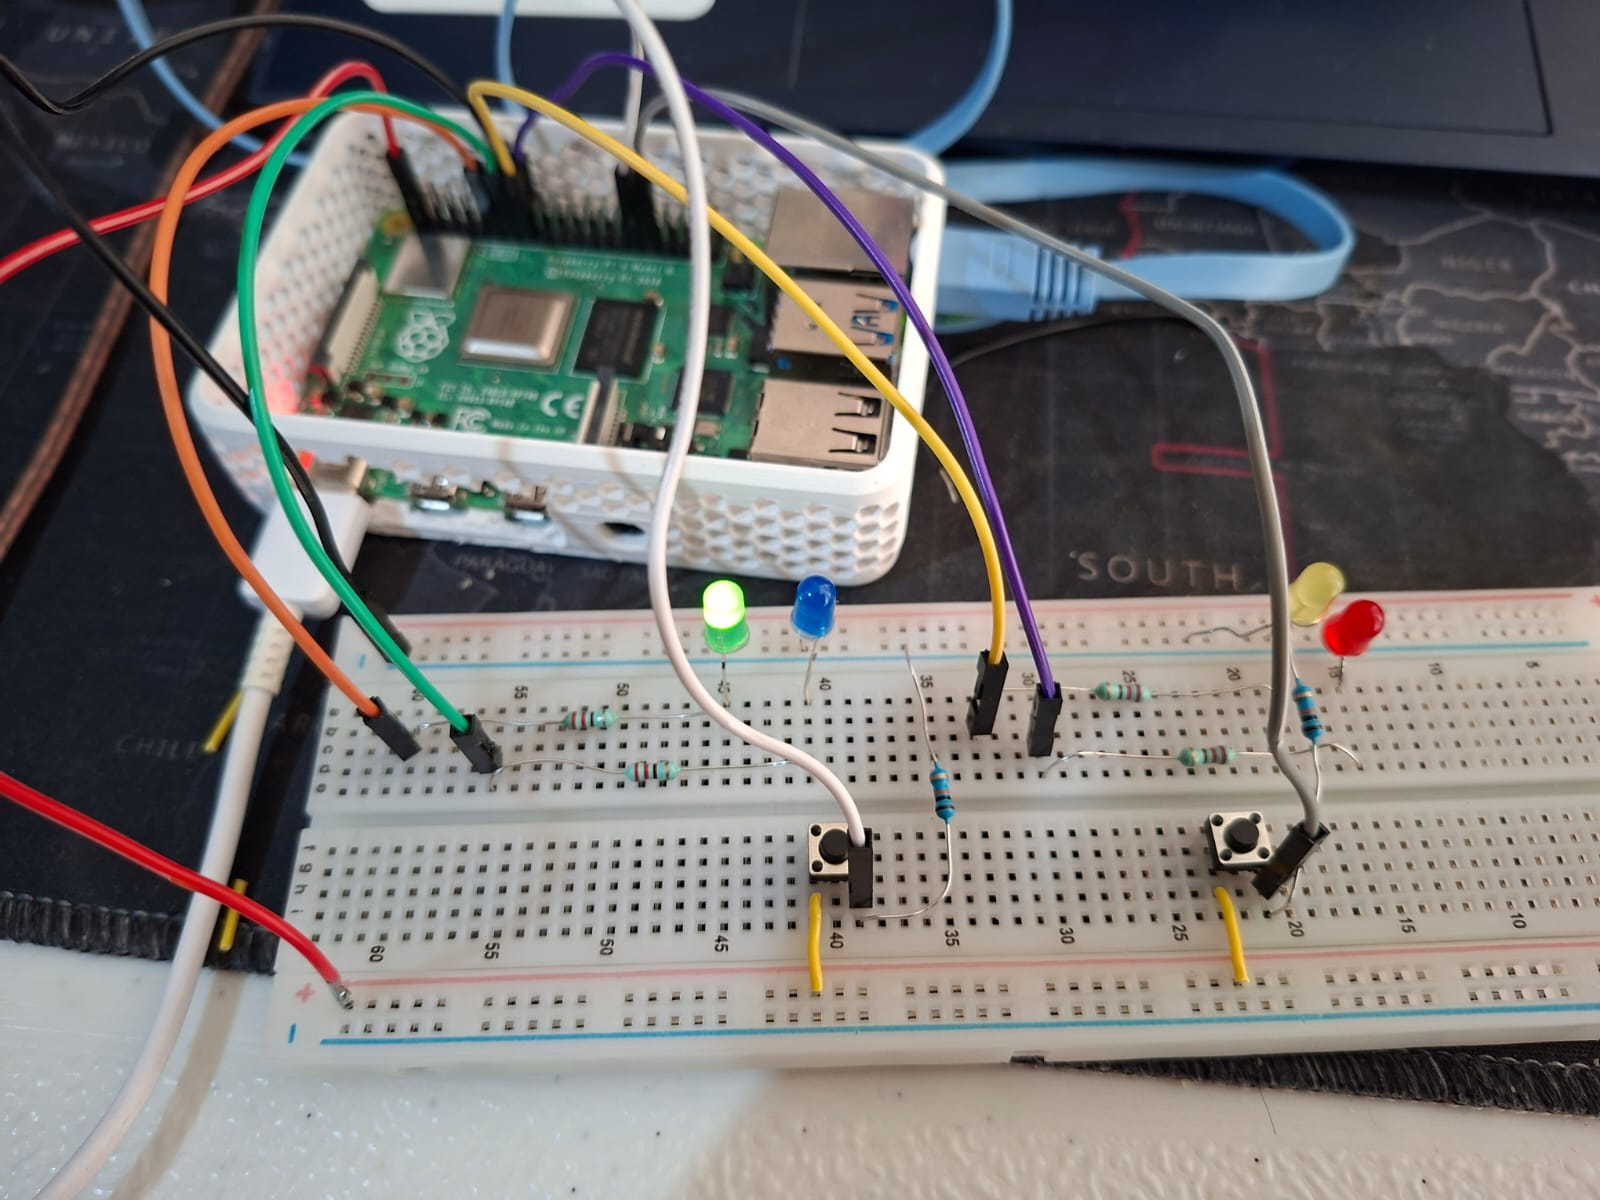
\includegraphics[width=\columnwidth]{img/fig00_circuito.jpg}
	\caption{Circuito armado en protoboard: cuatro LEDs con sus resistencias en serie y dos botones con resistencia \textit{pull-down}, conectados al \textit{header} de la Raspberry Pi 4.}
	\label{fig:circuito}
\end{figure}

\subsubsection{Parte B: Exploración desde la terminal}
Sin escribir código todavía, se utilizaron las herramientas de línea de comandos de \texttt{libgpiod}. Primero se listaron los chips y las líneas disponibles.

\begin{lstlisting}[language=bash,caption={Listado de chips y líneas GPIO.}]
gpioinfo
\end{lstlisting}

\begin{figure}[t]
	\centering
	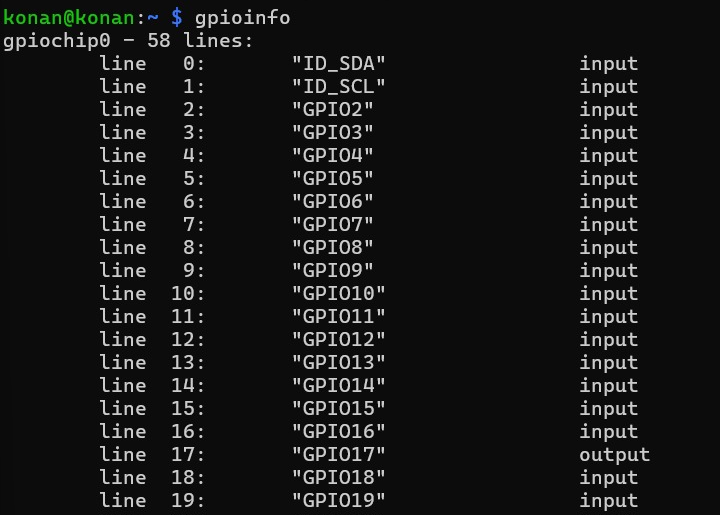
\includegraphics[width=\columnwidth]{img/fig01_gpioinfo.png}
	\caption{Salida de \texttt{gpioinfo} (líneas 0 a 19): el \texttt{gpiochip0} expone 58 líneas en total; la línea 17 aparece como \texttt{output} y las demás como \texttt{input}.}
	\label{fig:gpioinfo}
\end{figure}

Enseguida se encendió y apagó el LED 1 directamente desde la terminal. En la versión de \texttt{gpioset} instalada, la opción \texttt{-p 3s} mantiene el valor durante tres segundos antes de que la herramienta termine.

\begin{lstlisting}[language=bash,caption={Control del LED 1 con \texttt{gpioset}.}]
gpioset -c gpiochip0 -p 3s 17=1
\end{lstlisting}

\begin{figure}[t]
	\centering
	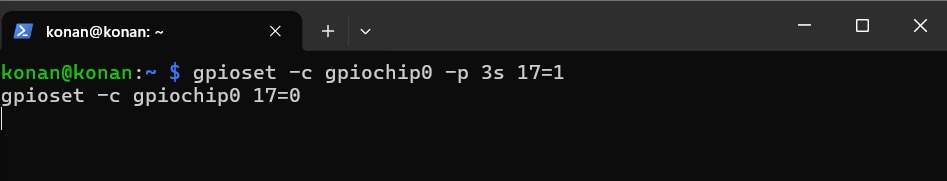
\includegraphics[width=\columnwidth]{img/fig02_gpioset.jpg}
	\caption{Encendido del LED 1 (GPIO17) durante 3~s con \texttt{gpioset}. La herramienta imprime el estado al que regresa la línea (\texttt{17=0}).}
	\label{fig:gpioset}
\end{figure}

Por último se leyó el botón 1 dos veces: una sin presionar y otra presionándolo durante la lectura.

\begin{lstlisting}[language=bash,caption={Lectura del botón 1 con \texttt{gpioget}.}]
gpioget --numeric -c gpiochip0 -p 3s 5
\end{lstlisting}

\begin{figure}[t]
	\centering
	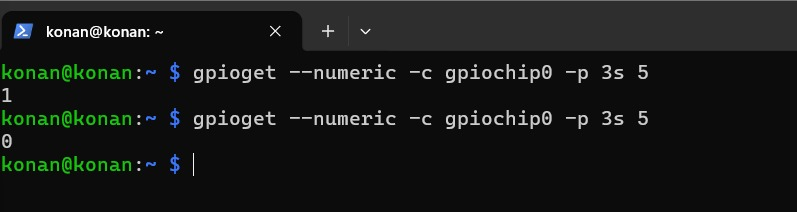
\includegraphics[width=\columnwidth]{img/fig03_gpioget.jpg}
	\caption{Lecturas del botón 1 (GPIO5): \texttt{1} con el botón presionado y \texttt{0} sin presionar.}
	\label{fig:gpioget}
\end{figure}

\begin{figure}[t]
	\centering
	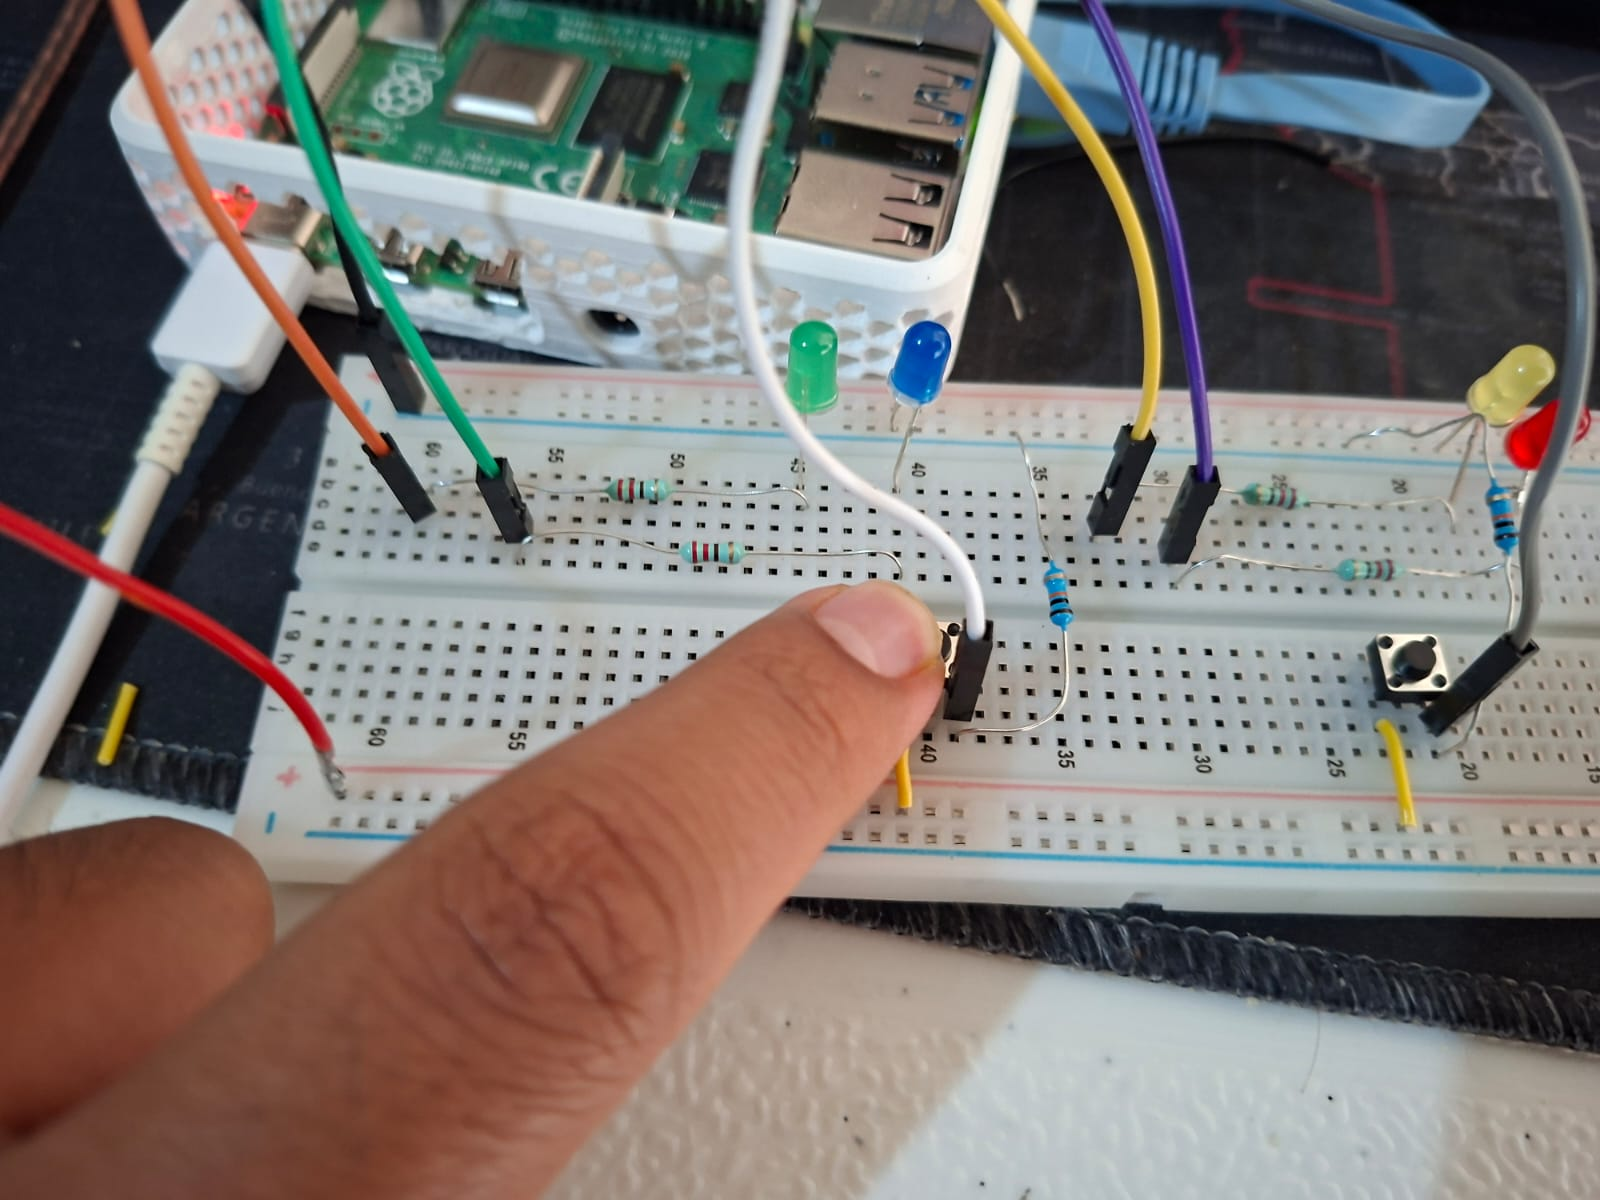
\includegraphics[width=\columnwidth]{img/fig04_dedo_boton.jpg}
	\caption{Presión del botón 1 durante la lectura con \texttt{gpioget}.}
	\label{fig:dedoboton}
\end{figure}

\subsubsection{Parte C: LEDs desde C}
Se escribió el programa \texttt{leds.c}, que recorre los cuatro LEDs en un patrón de ida y vuelta (tipo \textit{ping-pong}) durante tres rondas. El programa emplea la API v2 de \texttt{libgpiod}: se abre el chip con \texttt{gpiod\_chip\_open()}, se define una configuración de línea de salida con valor inicial inactivo y se solicitan las cuatro líneas en una sola petición (\texttt{gpiod\_chip\_request\_lines()}). Después, cada LED se enciende, se espera 200~ms con \texttt{usleep()} y se apaga.

\begin{lstlisting}[language=C,caption={Código fuente de \texttt{leds.c}.}]
#include <gpiod.h>
#include <stdio.h>
#include <unistd.h>

#define CHIP "/dev/gpiochip0"
#define N_LEDS 4
#define RONDAS 3

int main(void) {
	static const unsigned int pines[N_LEDS] = {17, 27, 22, 23};

	struct gpiod_chip *chip = gpiod_chip_open(CHIP);
	if (!chip) { perror("gpiod_chip_open"); return 1; }

	struct gpiod_line_settings *ajustes = gpiod_line_settings_new();
	gpiod_line_settings_set_direction(ajustes, GPIOD_LINE_DIRECTION_OUTPUT);
	gpiod_line_settings_set_output_value(ajustes, GPIOD_LINE_VALUE_INACTIVE);

	struct gpiod_line_config *cfg_lineas = gpiod_line_config_new();
	gpiod_line_config_add_line_settings(cfg_lineas, pines, N_LEDS, ajustes);

	struct gpiod_request_config *cfg_peticion = gpiod_request_config_new();
	gpiod_request_config_set_consumer(cfg_peticion, "leds");

	struct gpiod_line_request *peticion =
		gpiod_chip_request_lines(chip, cfg_peticion, cfg_lineas);
	if (!peticion) { perror("gpiod_chip_request_lines"); return 1; }

	for (int ronda = 0; ronda < RONDAS; ronda++) {
		for (int i = 0; i < N_LEDS; i++) {
			gpiod_line_request_set_value(peticion, pines[i], GPIOD_LINE_VALUE_ACTIVE);
			usleep(200000);
			gpiod_line_request_set_value(peticion, pines[i], GPIOD_LINE_VALUE_INACTIVE);
		}
		for (int i = N_LEDS - 2; i > 0; i--) {
			gpiod_line_request_set_value(peticion, pines[i], GPIOD_LINE_VALUE_ACTIVE);
			usleep(200000);
			gpiod_line_request_set_value(peticion, pines[i], GPIOD_LINE_VALUE_INACTIVE);
		}
	}

	/* Liberación de recursos */
	gpiod_line_request_release(peticion);
	gpiod_request_config_free(cfg_peticion);
	gpiod_line_config_free(cfg_lineas);
	gpiod_line_settings_free(ajustes);
	gpiod_chip_close(chip);
	return 0;
}
\end{lstlisting}

\begin{figure}[t]
	\centering
	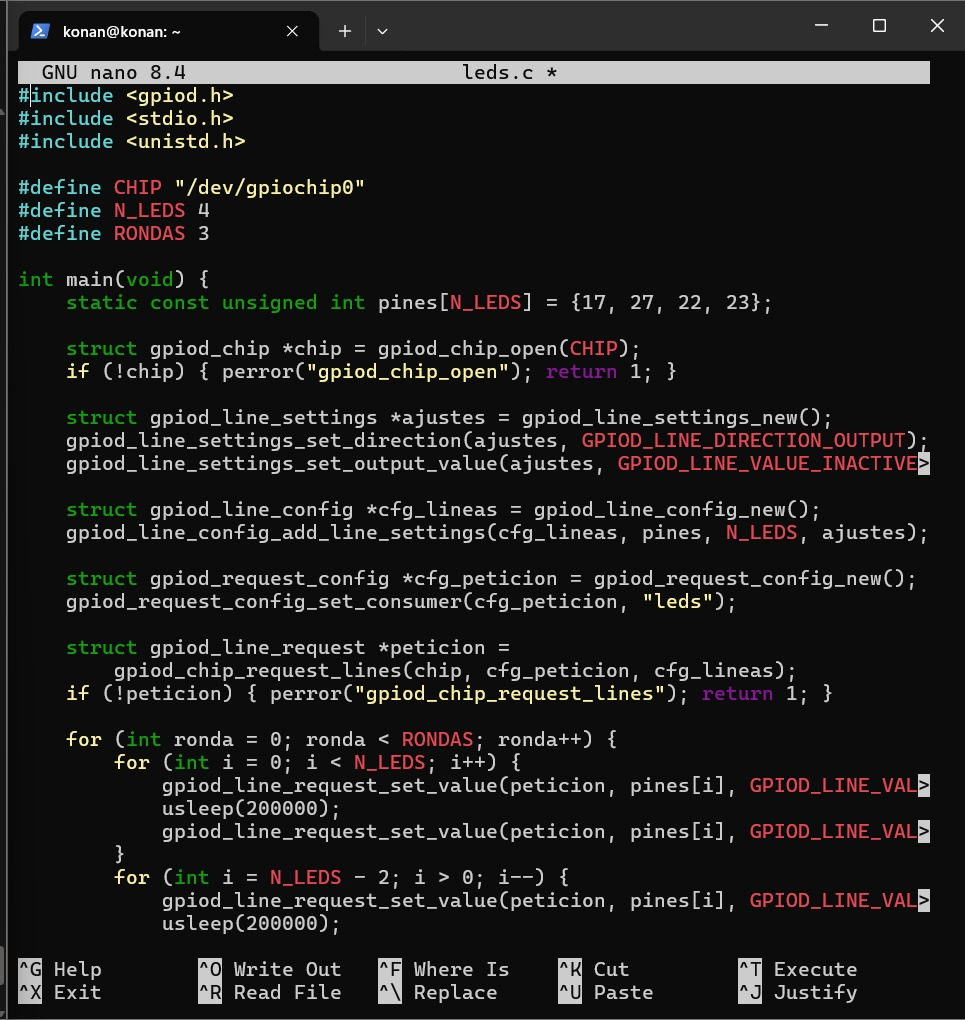
\includegraphics[width=\columnwidth]{img/fig06_leds_nano.jpg}
	\caption{Edición de \texttt{leds.c} en \texttt{nano}. Las líneas largas aparecen truncadas con \texttt{>} por el ancho de la terminal.}
	\label{fig:ledsnano}
\end{figure}

La compilación y ejecución se realizaron con la bandera \texttt{-lgpiod} al final del comando, requisito para que el enlazador resuelva los símbolos de la biblioteca.

\begin{lstlisting}[language=bash,caption={Compilación y ejecución de \texttt{leds.c}.}]
gcc leds.c -o leds -lgpiod
./leds
\end{lstlisting}

\begin{figure}[t]
	\centering
	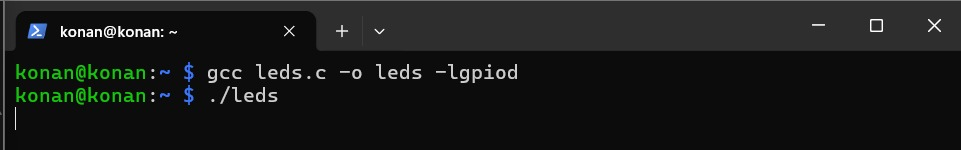
\includegraphics[width=\columnwidth]{img/fig07_gcc_leds.png}
	\caption{Compilación sin errores ni advertencias y ejecución de \texttt{leds}.}
	\label{fig:gccleds}
\end{figure}

\begin{figure*}[t]
	\centering
	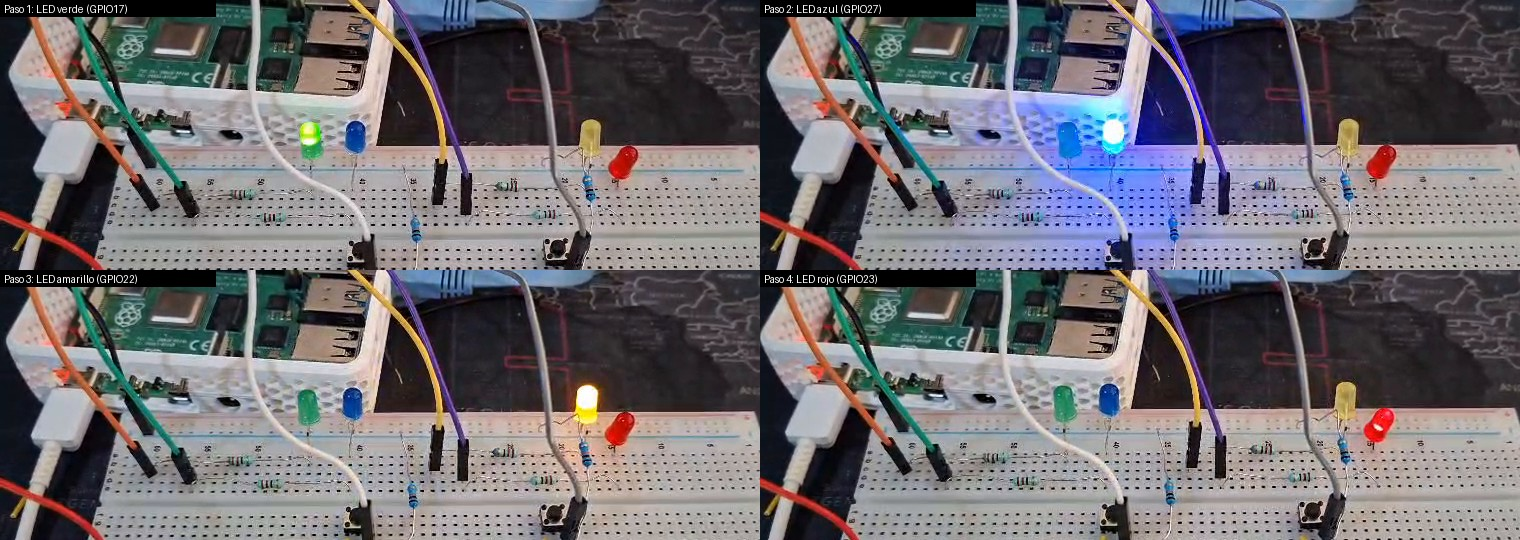
\includegraphics[width=\textwidth]{img/fig07b_leds_secuencia.jpg}
	\caption{Cuatro cuadros extraídos del video de la ejecución de \texttt{leds}: el LED encendido avanza del verde (GPIO17) al azul (GPIO27), al amarillo (GPIO22) y al rojo (GPIO23), siguiendo el orden del arreglo \texttt{pines}.}
	\label{fig:ledsecuencia}
\end{figure*}

\subsubsection{Parte D: Botón por \textit{polling}}
Se implementó \texttt{boton\_polling.c}, que lee continuamente el estado del botón 1 (GPIO5) y lo copia al LED 1 (GPIO17). Este programa se tomó de la guía de la práctica y utiliza la API v1 de \texttt{libgpiod}, distinta de la API v2 usada en \texttt{leds.c} y \texttt{semaforo.c}.

\begin{lstlisting}[language=C,caption={Código de \texttt{boton\_polling.c}.}]
#include <gpiod.h>
#include <stdio.h>

int main(void) {
	struct gpiod_chip *chip = gpiod_chip_open_by_name("gpiochip0");
	struct gpiod_line *boton = gpiod_chip_get_line(chip, 5);
	struct gpiod_line *led = gpiod_chip_get_line(chip, 17);

	gpiod_line_request_input(boton, "boton_polling");
	gpiod_line_request_output(led, "boton_polling", 0);

	while (1) {
		int estado = gpiod_line_get_value(boton);
		gpiod_line_set_value(led, estado);
	}
}
\end{lstlisting}

El núcleo del programa es el bucle \texttt{while (1)}, que no contiene ninguna espera: en cada iteración consulta el botón y escribe el LED, tan rápido como la CPU lo permite.

\begin{lstlisting}[language=bash,caption={Compilación y ejecución de \texttt{boton\_polling.c}.}]
gcc boton_polling.c -o boton_polling -lgpiod
./boton_polling
\end{lstlisting}

\begin{figure*}[t]
	\centering
	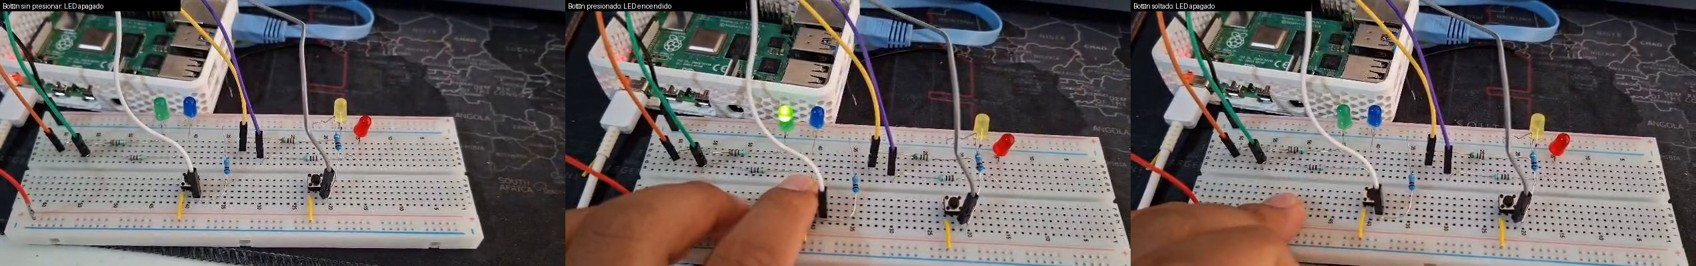
\includegraphics[width=\textwidth]{img/fig05_polling_video.jpg}
	\caption{Tres cuadros del video de \texttt{boton\_polling}: con el botón sin presionar el LED 1 permanece apagado; al presionarlo se enciende; al soltarlo se apaga.}
	\label{fig:pollingvideo}
\end{figure*}

En una segunda sesión SSH se ejecutó \texttt{top} para medir el costo de CPU mientras el programa estaba activo.

\begin{figure}[t]
	\centering
	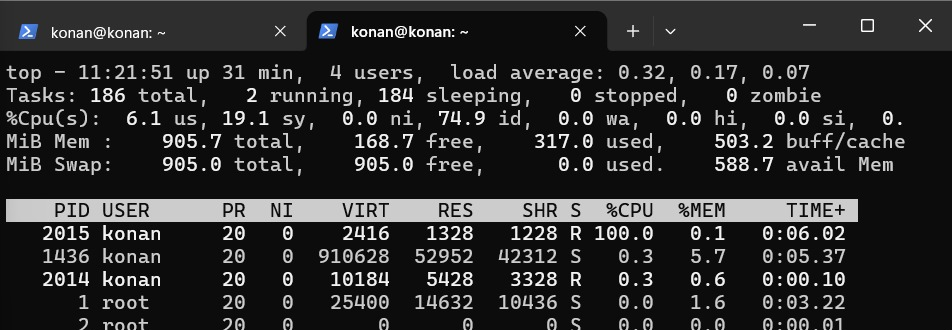
\includegraphics[width=\columnwidth]{img/fig08_top_polling.png}
	\caption{\texttt{top} con \texttt{boton\_polling} en ejecución (PID 2015): 100.0\,\% de CPU, estado \texttt{R}.}
	\label{fig:toppolling}
\end{figure}

\subsubsection{Parte E: El mismo botón, por eventos}
Se repitió la lectura del botón 1 con la herramienta \texttt{gpiomon}, que se suscribe a los flancos de la línea en lugar de consultarla repetidamente.

\begin{lstlisting}[language=bash,caption={Monitoreo por eventos con \texttt{gpiomon}.}]
gpiomon -c gpiochip0 5
\end{lstlisting}

\begin{figure}[t]
	\centering
	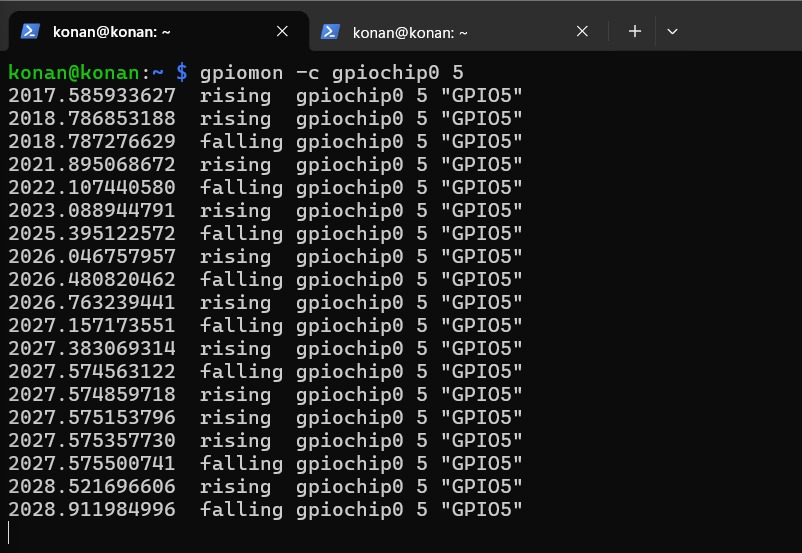
\includegraphics[width=\columnwidth]{img/fig09_gpiomon.jpg}
	\caption{Eventos registrados por \texttt{gpiomon} sobre GPIO5 al presionar y soltar el botón varias veces. Cada línea incluye la marca de tiempo del kernel en segundos.}
	\label{fig:gpiomon}
\end{figure}

\begin{figure}[t]
	\centering
	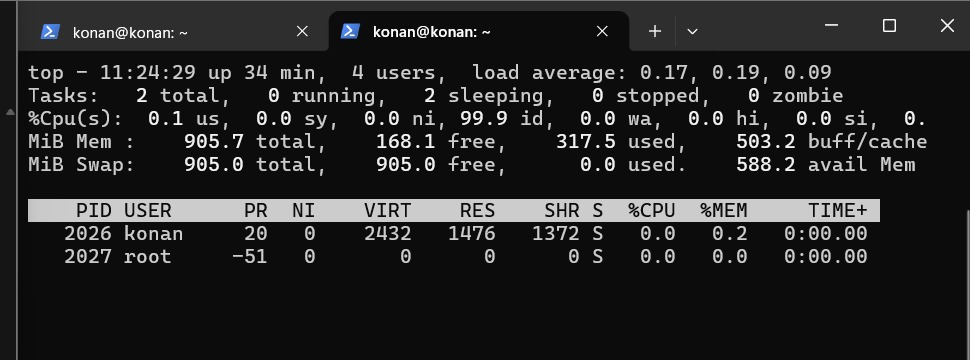
\includegraphics[width=\columnwidth]{img/fig10_top_gpiomon.jpg}
	\caption{\texttt{top} con \texttt{gpiomon} en espera (PID 2026): 0.0\,\% de CPU, estado \texttt{S}. Se observa además un proceso de \texttt{root} (PID 2027) con prioridad $-51$, también dormido.}
	\label{fig:topgpiomon}
\end{figure}

\subsubsection{Parte F: Reto final, semáforo peatonal}
Se diseñó \texttt{semaforo.c} desde cero, sin código de partida. Las reglas fueron: tres LEDs simulan un semáforo vehicular (rojo=GPIO17, amarillo=GPIO27, verde=GPIO22) con ciclo automático verde 5~s $\to$ amarillo 2~s $\to$ rojo 5~s; el botón 1 (GPIO5) es la petición de cruce, y al presionarlo el semáforo debe terminar su fase actual de forma segura y permanecer en rojo 8~s antes de reanudar; y el LED 4 (GPIO23) parpadea mientras el semáforo esté en rojo por petición peatonal, como indicador de cruce seguro.

La decisión de diseño central fue emplear \textbf{eventos} y no \textit{polling}. El semáforo debe llevar el tiempo de cada fase y además parpadear el LED de cruce mientras espera, por lo que no puede quedarse ciego dentro de un \texttt{sleep()} (perdería pulsaciones) ni consumir un núcleo entero en un bucle de lectura. La función \texttt{gpiod\_line\_request\_wait\_edge\_events()} bloquea el proceso con un temporizador: el planificador no le asigna CPU hasta que vence el plazo o el kernel detecta un flanco real en GPIO5.

\begin{lstlisting}[language=C,caption={Código fuente de \texttt{semaforo.c}.}]
#include <gpiod.h>
#include <stdio.h>
#include <signal.h>
#include <time.h>

#define CHIP "/dev/gpiochip0"
#define ROJO      17
#define AMARILLO  27
#define VERDE     22
#define CRUCE     23
#define BOTON      5

#define T_VERDE     5000
#define T_AMARILLO  2000
#define T_ROJO      5000
#define T_PEATONAL  8000
#define T_PARPADEO   500

/* Decision de diseno: se usan EVENTOS, no polling.
   El semaforo debe llevar el tiempo de cada fase y parpadear el LED de cruce
   mientras espera, asi que no puede quedarse ciego en un sleep() ni quemar un
   nucleo en un bucle de lectura. wait_edge_events() bloquea el proceso con un
   temporizador: el planificador no le da CPU hasta que expira el plazo o el
   kernel detecta un flanco real en GPIO5. Costo en reposo: 0%. */

static volatile sig_atomic_t seguir = 1;

static void parar(int sig) { (void)sig; seguir = 0; }

static int64_t ahora_ms(void) {
	struct timespec ts;
	clock_gettime(CLOCK_MONOTONIC, &ts);
	return (int64_t)ts.tv_sec * 1000 + ts.tv_nsec / 1000000;
}

/* Espera `ms` completos. Si llega un flanco antes, levanta *peticion y sigue
   esperando el tiempo restante: la fase en curso nunca se acorta. */
static void esperar(struct gpiod_line_request *req,
                    struct gpiod_edge_event_buffer *buf,
                    int ms, int *peticion)
{
	int64_t fin = ahora_ms() + ms;
	int64_t restante;

	while (seguir && (restante = fin - ahora_ms()) > 0) {
		int r = gpiod_line_request_wait_edge_events(req, restante * 1000000);
		if (r > 0) {
			gpiod_line_request_read_edge_events(req, buf, 8);
			*peticion = 1;
		} else if (r < 0) {
			break;
		}
	}
}

static void luz(struct gpiod_line_request *req, unsigned int pin, int on) {
	gpiod_line_request_set_value(req, pin,
		on ? GPIOD_LINE_VALUE_ACTIVE : GPIOD_LINE_VALUE_INACTIVE);
}

int main(void) {
	static const unsigned int salidas[4] = {ROJO, AMARILLO, VERDE, CRUCE};
	static const unsigned int entradas[1] = {BOTON};

	signal(SIGINT, parar);

	struct gpiod_chip *chip = gpiod_chip_open(CHIP);
	if (!chip) { perror("gpiod_chip_open"); return 1; }

	struct gpiod_line_settings *cfg_out = gpiod_line_settings_new();
	gpiod_line_settings_set_direction(cfg_out, GPIOD_LINE_DIRECTION_OUTPUT);
	gpiod_line_settings_set_output_value(cfg_out, GPIOD_LINE_VALUE_INACTIVE);

	struct gpiod_line_settings *cfg_in = gpiod_line_settings_new();
	gpiod_line_settings_set_direction(cfg_in, GPIOD_LINE_DIRECTION_INPUT);
	gpiod_line_settings_set_edge_detection(cfg_in, GPIOD_LINE_EDGE_RISING);
	gpiod_line_settings_set_debounce_period_us(cfg_in, 20000);

	struct gpiod_line_config *lineas = gpiod_line_config_new();
	gpiod_line_config_add_line_settings(lineas, salidas, 4, cfg_out);
	gpiod_line_config_add_line_settings(lineas, entradas, 1, cfg_in);

	struct gpiod_request_config *cfg_pet = gpiod_request_config_new();
	gpiod_request_config_set_consumer(cfg_pet, "semaforo");

	struct gpiod_line_request *req =
		gpiod_chip_request_lines(chip, cfg_pet, lineas);
	if (!req) { perror("gpiod_chip_request_lines"); return 1; }

	struct gpiod_edge_event_buffer *buf = gpiod_edge_event_buffer_new(8);
	if (!buf) { perror("gpiod_edge_event_buffer_new"); return 1; }

	int peticion = 0;

	while (seguir) {
		luz(req, VERDE, 1); luz(req, AMARILLO, 0); luz(req, ROJO, 0);
		esperar(req, buf, T_VERDE, &peticion);
		if (!seguir) break;

		luz(req, VERDE, 0); luz(req, AMARILLO, 1);
		esperar(req, buf, T_AMARILLO, &peticion);
		if (!seguir) break;

		luz(req, AMARILLO, 0); luz(req, ROJO, 1);

		int cruce = peticion;
		peticion = 0;

		if (cruce) {
			int ciclos = T_PEATONAL / T_PARPADEO;
			for (int i = 0; i < ciclos && seguir; i++) {
				luz(req, CRUCE, i % 2 == 0);
				esperar(req, buf, T_PARPADEO, &peticion);
			}
			luz(req, CRUCE, 0);
		} else {
			esperar(req, buf, T_ROJO, &peticion);
		}
	}

	for (int i = 0; i < 4; i++) luz(req, salidas[i], 0);

	gpiod_edge_event_buffer_free(buf);
	gpiod_line_request_release(req);
	gpiod_request_config_free(cfg_pet);
	gpiod_line_config_free(lineas);
	gpiod_line_settings_free(cfg_in);
	gpiod_line_settings_free(cfg_out);
	gpiod_chip_close(chip);
	return 0;
}
\end{lstlisting}

\begin{figure*}[t]
	\centering
	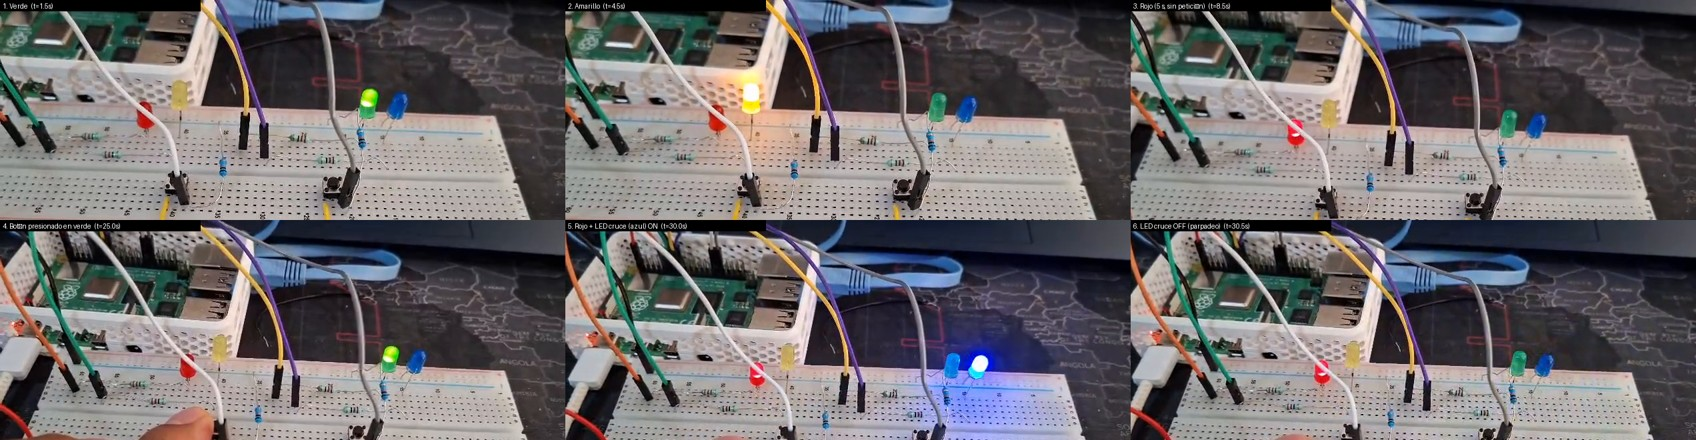
\includegraphics[width=\textwidth]{img/fig11_semaforo.jpg}
	\caption{Cuadros del video de \texttt{semaforo} en la Raspberry Pi. En esta toma la cámara está del lado opuesto al de las fotos anteriores: el LED rojo queda a la izquierda y los LEDs verde y azul a la derecha. El rojo se ve tenue por la exposición de la cámara.}
	\label{fig:semaforo}
\end{figure*}

\subsubsection{Parte G: Commit con Git}
Los archivos fuente de la práctica se agregaron al mismo repositorio de la Práctica 1.

\begin{lstlisting}[language=bash,caption={Registro de la práctica en Git.}]
git add leds.c boton_polling.c semaforo.c
git commit -m "Practica 2: GPIO"
git log --oneline
\end{lstlisting}

\begin{figure}[t]
	\centering
	\imgph{Salida de \texttt{git log -{}-oneline} mostrando el commit de la Práctica 2}{3.5cm}
	\caption{Historial del repositorio con el commit de la Práctica 2.}
	\label{fig:gitlog}
\end{figure}

\section{Resultados y Análisis}

\subsection{Exploración desde la terminal}
\texttt{gpioinfo} (Fig.~\ref{fig:gpioinfo}) reportó un único chip, \texttt{gpiochip0}, con 58 líneas. Las líneas 0 y 1 aparecen con los nombres \texttt{ID\_SDA} e \texttt{ID\_SCL}, que corresponden a los pines reservados para la identificación de \textit{HATs} (por eso solo 26 de los 28 GPIO del \textit{header} son de uso libre). En la salida completa (no recortada en la Fig.~\ref{fig:gpioinfo}) figuran además líneas que no pertenecen al \textit{header} de 40 pines sino a periféricos de la placa, como \texttt{RGMII\_MDIO} y \texttt{RGMIO\_MDC} (Ethernet), \texttt{CTS0}/\texttt{RTS0}/\texttt{TXD0}/\texttt{RXD0} (UART) y \texttt{SD1\_*} (tarjeta SD). Es decir, el chip expone todas las líneas del SoC, no solo las del \textit{header}.

En la captura, la línea 17 figura como \texttt{output} y las demás como \texttt{input}. La dirección de una línea no es una propiedad fija del pin sino un estado que el software configura; \texttt{gpioinfo} refleja ese estado en el momento de la consulta.

En \texttt{gpioget} (Fig.~\ref{fig:gpioget}) la primera lectura devolvió \texttt{1} con el botón presionado y la segunda \texttt{0} con el botón suelto, lo cual confirma el funcionamiento de la resistencia \textit{pull-down}: el pin lee 0 en reposo, porque la resistencia de 10~k$\Omega$ lo mantiene conectado a tierra, y 1 únicamente cuando el botón lo conecta a 3.3~V.

\subsection{Patrón de LEDs}
\texttt{leds.c} compiló sin advertencias y el patrón se observó en las cuatro salidas (Fig.~\ref{fig:ledsecuencia}). El orden de encendido siguió el del arreglo \texttt{pines = \{17, 27, 22, 23\}}, lo que confirma la correspondencia entre color y GPIO de la Tabla~\ref{tab:conexion}.

Vale la pena analizar el segundo bucle del programa. El primero recorre los índices 0, 1, 2, 3 (ida). El segundo arranca en \texttt{N\_LEDS - 2}, es decir, en el índice 2, y baja hasta el 1 sin llegar a 0. Con ello el patrón completo de una ronda es 0, 1, 2, 3, 2, 1, y la siguiente ronda comienza de nuevo en 0. Si la vuelta incluyera los extremos, el LED de cada punta se encendería dos veces seguidas y el movimiento se vería con una pausa; al excluirlos, el barrido es continuo. Cada ronda dura
\begin{equation}
	t_{ronda} = 6~\text{encendidos} \times 0.2~\text{s} = 1.2~\text{s},
\end{equation}
y tres rondas suman 3.6~s, sin contar el tiempo de las llamadas al sistema.

Además, el programa solicita las cuatro líneas en una única llamada a \texttt{gpiod\_chip\_request\_lines()}. En la API v2 una petición es un objeto que agrupa varias líneas con su configuración, de modo que un solo \texttt{set\_value} puede dirigirse a cualquiera de ellas por su número de \textit{offset}. Esto es más eficiente que la API v1, que exigía obtener y solicitar cada línea por separado.

\subsection{\textit{Polling} contra eventos}
Este es el resultado central de la práctica, y se resume en la Tabla~\ref{tab:cpu}.

\begin{table}[t]
	\centering
	\caption{Costo de CPU de las dos estrategias de lectura del botón.}
	\label{tab:cpu}
	\begin{tabular}{|l|c|c|c|}
		\hline
		\textbf{Estrategia} & \textbf{\%CPU} & \textbf{Estado} & \textbf{CPU inactiva} \\
		\hline
		\texttt{boton\_polling} & 100.0 & R (ejecución) & 74.9\,\% \\
		\hline
		\texttt{gpiomon} (eventos) & 0.0 & S (dormido) & 99.9\,\% \\
		\hline
	\end{tabular}
\end{table}

Con \texttt{boton\_polling} (Fig.~\ref{fig:toppolling}) el proceso ocupó el 100.0\,\% de CPU y su estado fue \texttt{R}. Con \texttt{gpiomon} (Fig.~\ref{fig:topgpiomon}) ocupó 0.0\,\% y su estado fue \texttt{S}; \texttt{top} reportó además dos tareas totales frente a las 186 de la medición anterior, porque la segunda medición se filtró por proceso. La diferencia se explica por el diseño de cada uno. El bucle de \texttt{boton\_polling} no contiene ninguna espera, de manera que jamás cede el procesador voluntariamente y el planificador lo mantiene en ejecución hasta agotar cada porción de tiempo. \texttt{gpiomon}, en cambio, solicita al kernel que lo despierte solo cuando ocurra un flanco; mientras tanto el proceso se bloquea y el planificador le asigna CPU cero.

Un detalle sutil: la línea de resumen de CPU de la Fig.~\ref{fig:toppolling} indica 74.9\,\% inactivo, no 0\,\%. Esto se debe a que la Raspberry Pi 4 tiene cuatro núcleos y \texttt{top} promedia el porcentaje entre todos ellos por defecto. El proceso de polling satura un único núcleo, que equivale al 25\,\% del total del sistema, y por eso el resto del CPU aparece como libre. El 100.0\,\% de la columna \texttt{\%CPU} es relativo a un núcleo, mientras que el 74.9\,\% de inactividad es relativo al sistema completo; ambas cifras son consistentes entre sí.

En la Fig.~\ref{fig:topgpiomon} aparece, junto a \texttt{gpiomon}, un segundo proceso del usuario \texttt{root} (PID 2027) con prioridad $-51$ y estado \texttt{S}, también sin consumo de CPU. Solo se registra como observación: la captura no permite determinar su función. Lo relevante es que, con eventos, quien espera está dormido y el kernel despierta al proceso únicamente cuando hay un cambio real en la línea.

Se destaca una segunda consecuencia del polling que no aparece en la tabla. Mientras \texttt{boton\_polling} consume un núcleo completo para hacer una sola tarea trivial, un sistema embebido con más responsabilidades, como llevar el tiempo de las fases de un semáforo, no podría permitírselo. Con eventos, el mismo hilo queda libre para otras tareas o para dormir, con el consiguiente ahorro de energía, algo relevante en dispositivos alimentados por batería.

\subsection{Rebote mecánico del botón}
La traza de \texttt{gpiomon} (Fig.~\ref{fig:gpiomon}) contiene un hallazgo que no estaba previsto en la guía: el \textbf{rebote} (\textit{bouncing}) del botón. Un botón mecánico no conmuta limpiamente; al cerrarse, sus contactos vibran y generan varias transiciones rápidas antes de estabilizarse. Es visible en los eventos de las marcas 2027.574563 a 2027.575500 (Tabla~\ref{tab:rebote}):

\begin{table}[t]
	\centering
	\caption{Ráfaga de eventos por rebote en \texttt{gpiomon} (marcas de tiempo en segundos).}
	\label{tab:rebote}
	\begin{tabular}{|c|c|c|}
		\hline
		\textbf{Marca de tiempo} & \textbf{Flanco} & \textbf{$\Delta t$ desde el anterior} \\
		\hline
		2027.574563 & falling & --- \\
		\hline
		2027.574859 & rising & 0.30~ms \\
		\hline
		2027.575153 & rising & 0.29~ms \\
		\hline
		2027.575357 & rising & 0.20~ms \\
		\hline
		2027.575500 & falling & 0.14~ms \\
		\hline
	\end{tabular}
\end{table}

En menos de 1~ms el pin registró cinco transiciones, con tres flancos \texttt{rising} seguidos sin un \texttt{falling} intermedio. Para una pulsación humana, que dura cientos de milisegundos (por ejemplo, la observada entre 2026.480820 y 2026.763239, de unos 0.28~s), una ráfaga de $\sim$1~ms es ruido de conmutación y no una pulsación real.

Esto tiene una consecuencia directa sobre el diseño del semáforo. Si el programa contara cada flanco como una petición, un solo botonazo podría interpretarse como varios. Por eso \texttt{semaforo.c} configura un periodo de antirrebote del kernel con \texttt{gpiod\_line\_settings\_set\_debounce\_period\_us(cfg\_in, 20000)}, es decir, 20~ms: el kernel ignora los flancos que ocurran dentro de esa ventana tras el primero. El valor de 20~ms es holgado respecto de la ráfaga de $\sim$1~ms observada y muy inferior a la duración de una pulsación humana, por lo que filtra el rebote sin perder pulsaciones legítimas. Además, el antirrebote lo realiza el kernel en lugar del programa, lo que evita contar el tiempo en el espacio de usuario.

\subsection{Semáforo peatonal}
El diseño de \texttt{semaforo.c} descansa en la función \texttt{esperar()}, cuya propiedad clave es que \textbf{nunca acorta una fase}. Si llega un flanco durante el plazo, solo se levanta la bandera \texttt{peticion} y el bucle continúa esperando el tiempo restante hasta el vencimiento. Esto cumple literalmente el requisito de \textit{terminar su fase actual de forma segura}: un peatón que presiona el botón durante el verde o el amarillo no interrumpe la fase, sino que el semáforo la completa y recién entonces concede el cruce.

El comportamiento se verificó sobre el hardware analizando el video de la ejecución cuadro por cuadro (Fig.~\ref{fig:semaforo}). Se muestreó a 4 cuadros por segundo, por lo que cada tiempo tiene una incertidumbre de $\pm 0.25$~s, y se detectó automáticamente qué LED estaba encendido en cada cuadro. Los resultados se resumen en la Tabla~\ref{tab:fases}.

\begin{table}[t]
	\centering
	\caption{Fases medidas en el video del semáforo ($\pm 0.25$~s).}
	\label{tab:fases}
	\footnotesize
	\begin{tabular}{|l|c|c|}
		\hline
		\textbf{Fase} & \textbf{Intervalo (s)} & \textbf{Duración (s)} \\
		\hline
		Amarillo & 4.0 -- 6.0 & 2.0 \\
		\hline
		Rojo (sin petición) & 6.0 -- 11.0 & 5.0 \\
		\hline
		Verde & 11.0 -- 16.0 & 5.0 \\
		\hline
		Amarillo & 16.0 -- 18.0 & 2.0 \\
		\hline
		Rojo (sin petición) & 18.0 -- 23.0 & 5.0 \\
		\hline
		Verde & 23.0 -- 28.0 & 5.0 \\
		\hline
		Amarillo & 28.0 -- 30.0 & 2.0 \\
		\hline
		Rojo + cruce (LED 4 parpadea) & 30.0 -- $\approx$38.0 & $\approx$8.0 \\
		\hline
	\end{tabular}
\end{table}

La primera fase de verde no se incluye porque el video ya iniciaba con ella en curso. Todas las duraciones coinciden con las reglas de la práctica: verde 5~s, amarillo 2~s, rojo 5~s y rojo peatonal 8~s.

En el video se observa el dedo sobre el botón alrededor de $t=24$--$27$~s, durante la fase de verde que comienza en $t=23$~s. El semáforo no interrumpe esa fase: completa el verde (hasta $t=28$~s) y el amarillo (hasta $t=30$~s), y solo entonces entra en el rojo peatonal. Esto confirma en hardware la propiedad de que \texttt{esperar()} nunca acorta una fase. Durante el rojo peatonal el LED de cruce se enciende y apaga alternadamente: se contaron 7 destellos completos entre $t=30$ y $t=37.5$~s (Fig.~\ref{fig:semaforo}), y en la fracción restante el video termina con el ciclo ya reiniciado en verde. Con $T_{PARPADEO}=500$~ms el periodo de parpadeo es de 1~s, consistente con lo observado.

El video solo cubre una pulsación durante el verde. El comportamiento ante una pulsación durante el rojo normal, que no se probó en hardware, se deduce del código y es una decisión de implementación que no dictan las reglas de la práctica. La variable \texttt{peticion} se copia a \texttt{cruce} y se reinicia en cero justo al inicio del rojo; a partir de ahí, \texttt{esperar()} sigue recibiendo la dirección de \texttt{peticion}, por lo que cualquier pulsación posterior queda registrada para el siguiente ciclo. La consecuencia es que un peatón que llega cuando el semáforo ya está en rojo (sin haber pulsado antes) no obtiene cruce en ese rojo, sino en el próximo. Una alternativa habría sido permitir extender el rojo de 5~s a 8~s si la pulsación llega dentro de él, pero eso alteraría la duración del rojo por una pulsación tardía; se optó por el comportamiento más conservador que garantiza que ninguna fase se acorte ni se prolongue de manera no anunciada.

En el rojo por petición, el LED de cruce parpadea con \texttt{i \% 2 == 0}: el programa ejecuta $T_{PEATONAL}/T_{PARPADEO} = 8000/500 = 16$ iteraciones de 500~ms, enciende el LED en las iteraciones pares y lo apaga en las impares, de modo que el LED emite 8 destellos de 500~ms de encendido y 500~ms de apagado, con periodo de 1~s. Al terminar, \texttt{luz(req, CRUCE, 0)} garantiza que el LED quede apagado.

Otros detalles de robustez del programa: el manejador \texttt{parar()} de \texttt{SIGINT} solo asigna una bandera de tipo \texttt{volatile sig\_atomic\_t}, el único tipo cuya lectura y escritura está garantizada como segura en un manejador de señales; el bucle principal la consulta y, al terminar, apaga los cuatro LEDs y libera cada objeto de \texttt{libgpiod} en orden inverso al de su creación. Asimismo, el reloj empleado es \texttt{CLOCK\_MONOTONIC}, que no se ve afectado por ajustes de la hora del sistema, importante en un equipo que, como se vio en la Práctica 1, arranca sin reloj de tiempo real y sincroniza la hora por NTP después de iniciar.

\subsection{Problemas encontrados}

\begin{table}[t]
	\centering
	\caption{Incidencias potenciales y su solución.}
	\label{tab:problemas}
	\begin{tabular}{|p{3.3cm}|p{4.1cm}|}
		\hline
		\textbf{Problema} & \textbf{Solución aplicada} \\
		\hline
		Los archivos de la guía usan la API v1 de \texttt{libgpiod}, pero el paquete instalado en la Pi corresponde a la API v2. & \texttt{leds.c} y \texttt{semaforo.c} se escribieron con la API v2 (\texttt{gpiod\_chip\_open}, \texttt{line\_settings}). \\
		\hline
		Un solo botonazo genera varios flancos por rebote mecánico. & Antirrebote del kernel de 20~ms en \texttt{semaforo.c}. \\
		\hline
		Error de enlace \texttt{undefined reference to gpiod\_...}. & Colocar \texttt{-lgpiod} al final del comando \texttt{gcc}. \\
		\hline
	\end{tabular}
\end{table}

\section{Conclusiones}

\textbf{Belmont Muñoz Samuel}. Esta práctica permitió comprender de manera práctica y directa el control de hardware desde software, entendiendo que un pin GPIO no es más que un voltaje controlado eléctricamente dentro de límites muy específicos. Resultó fundamental aplicar correctamente los cálculos de resistencias para proteger los pines de la Raspberry Pi, evitando daños por exceso de corriente. La comparación experimental entre polling y eventos demostró contundentemente que un diseño basado en lectura continua puede desperdiciar recursos del procesador de forma innecesaria, mientras que el enfoque por eventos permite que el kernel gestione eficientemente las interrupciones. Finalmente, la implementación del semáforo peatonal integró todos los conceptos de la práctica, desde el control de múltiples salidas hasta la lectura segura de entradas con antirrebote, estableciendo una base sólida para el trabajo con sistemas embebidos más complejos.

\textbf{Domínguez Palacios Jesús Alejandro}. Lo más revelador de esta práctica fue medir con \texttt{top} la diferencia entre polling (100\,\% de CPU) y eventos (0\,\% de CPU) sobre hardware real, porque confirma que leer GPIO en bucle cerrado no solo consume recursos sino que literalmente satura un núcleo completo para una tarea que debería costar cero. El cálculo de la resistencia de 220~$\Omega$ para limitar la corriente del LED a unos 5.9~mA me dejó claro que los 16~mA máximos del pin no son un número arbitrario sino un límite eléctrico real que, de violarse, puede dañar el SoC de forma permanente. La elección de \texttt{libgpiod} tampoco fue accidental: bibliotecas como \texttt{RPi.GPIO} dejaron de funcionar en la Raspberry Pi 5 porque acceden directamente a registros del SoC, mientras que \texttt{libgpiod} se comunica con el kernel a través de \texttt{/dev/gpiochipN} y por eso el mismo código en C funciona en ambos modelos. El rebote del botón, visible en la ráfaga de cinco flancos en menos de 1~ms, mostró que un interruptor mecánico no conmuta limpiamente y que confiar en el antirrebote por hardware del kernel con 20~ms es más robusto que filtrar manualmente en el espacio de usuario. Finalmente, el diseño de \texttt{esperar()} en el semáforo, que nunca acorta una fase aunque llegue un evento, garantiza la seguridad del cruce por construcción y no por buena suerte.

\textbf{Dorantes Mejía Emmanuel}. En esta práctica aprendí de forma concreta cómo controlar hardware utilizando GPIO y la importancia de proteger los pines con resistencias adecuadas para evitar daños a la Raspberry Pi. Pude comprender mejor la diferencia entre polling y eventos al medir el uso de CPU: mientras que polling consume el 100\% de un núcleo sin hacer nada útil, el enfoque basado en eventos permite que el kernel despierte el proceso solo cuando ocurre un cambio real, optimizando completamente los recursos. También fue interesante observar el fenómeno del rebote mecánico del botón y cómo el kernel puede filtrar automáticamente esos rebotes mediante configuración por software, evitando conteos erróneos. La implementación del semáforo peatonal permitió integrar todo lo aprendido: controlar múltiples LEDs, leer botones de forma eficiente y garantizar tiempos de seguridad en cada fase. 

\textbf{García Olvera Emiliano}. En esta práctica se vio que un pin GPIO es solo un voltaje que el software decide leer o escribir, y que la calidad del programa depende de cómo se espera ese voltaje. Diseñar el semáforo obligó a escoger entre polling y eventos con un criterio real: como el programa tiene que contar el tiempo de cada fase y parpadear el LED de cruce, un bucle de lectura habría ocupado un núcleo entero y un \texttt{sleep()} habría hecho perder pulsaciones, así que la elección por eventos fue prácticamente obligada. Lo que más rescato es que \texttt{esperar()} nunca acorta una fase, de modo que la seguridad del cruce queda garantizada por construcción.

\textbf{Hernández Alonso Antonio Adonahí}. Esta práctica demostró que controlar hardware desde software no es magia sino electricidad bien entendida. Calcular la resistencia de 220~$\Omega$ para proteger el pin GPIO del LED confirmó que los límites de corriente son reales y que ignorarlos daña componentes. Usar \texttt{libgpiod} en lugar de acceso directo a registros mostró la ventaja de abstracciones del kernel: el mismo código funciona sin cambios entre versiones. La comparación entre polling (100\% CPU) y eventos (0\% CPU) fue contundente: esperar activamente desperdicia un núcleo completo, mientras que los eventos del kernel solo despiertan el proceso cuando ocurre un cambio real. Implementar el semáforo peatonal integró todo: control de múltiples LEDs, lectura de botón por eventos, temporización con \texttt{clock\_gettime()}, y lógica de estados que garantiza tiempos mínimos de seguridad. El antirrebote por hardware del kernel simplificó el código al eliminar filtrado manual. Esta arquitectura basada en eventos es directamente aplicable a sistemas embebidos donde eficiencia energética y respuesta en tiempo real son críticas.

\textbf{Jiménez Reyes Alan Yael}. Durante esta práctica pude aplicar el control a bajo nivel del hardware mediante la Raspberry Pi utilizando la librería libgpiod. Comprendí la vital importancia de no sobrepasar el límite de 3.3V y 16mA por pin para salvaguardar la integridad de la placa. Lo más interesante fue observar en tiempo real, gracias a la herramienta top, cómo un mal diseño de software basado en polling puede desperdiciar recursos del procesador, y cómo el enfoque por eventos soluciona este problema eficientemente. Finalmente, implementar el semáforo me ayudó a consolidar la lógica de programación integrando múltiples salidas y entradas al mismo tiempo.

\begin{thebibliography}{00}
	\bibitem{libgpiod} Linux GPIO subsystem. (2024). ``GPIO Character Device Userspace API'', \textit{Linux Kernel Documentation}. Disponible en: https://www.kernel.org/doc/html/latest/userspace-api/gpio/
	\bibitem{rpi_gpio} Raspberry Pi Ltd. (2024). ``Raspberry Pi Documentation --- GPIO and the 40-pin header'', Disponible en: https://www.raspberrypi.com/documentation/computers/raspberry-pi.html
	\bibitem{libgpiod_docs} B. Golaszewski. (2024). ``libgpiod --- C library and tools for interacting with the linux GPIO character device'', Disponible en: https://git.kernel.org/pub/scm/libs/libgpiod/libgpiod.git/
	\bibitem{gnu_toolchain} Free Software Foundation. (2024). ``GCC, the GNU Compiler Collection'', \textit{GNU Project}. Disponible en: https://gcc.gnu.org/
	\bibitem{git_scm} S. Chacon y B. Straub. (2014). \textit{Pro Git}, 2a ed. Apress. Disponible en: https://git-scm.com/book/
\end{thebibliography}

\end{document}
